\section{Neutron Diffusion Results}
\label{sec:diffusionResults}

\begin{frame}{One-Dimension, One-Group, Fixed Source}
  \begin{table}
    %\caption{One-Dimension, One-Group, Fixed Source Convergence Study 
    %  Results.}
    \label{tab:1dfixedsrc}
    \begin{center}
      \begin{tabular}{ccccc}
        \toprule
        Refine & RMS & RMS ratio & $\|e\|_{\infty}$ & 
          $\|e\|_{\infty}$ ratio \\
        \midrule
        \csvreader[
          late after line=\\,
          late after last line=\\\bottomrule,]
          {../ch03_diffusionResults/data/1dfixedsrc.csv}{}
          {\csvcoli & \csvcolii & \csvcoliii & \csvcolviii & \csvcolix}
      \end{tabular}
    \end{center}
  \end{table}
  \begin{equation}
    \label{eq:analytic_1dfixedsrc}
    \phi(x) = \left( \frac{q_{fixed}}{D} \right) 
      \left( 1-\cosh(\kappa\,x) +
      \frac{\cosh(\kappa\,L_x)-1}{\sinh(\kappa\,L_x)}
      \sinh(\kappa\,x)\right)
  \end{equation}
\end{frame}

\begin{frame}{One-Dimension, One-Group, Criticality}
  \begin{table}
    %\caption{One-Dimension, One-Group, Criticality Convergence Study
    %  Results.}
    \label{tab:1d1g}
    \begin{center}
      \resizebox{\textwidth}{!}{
      \begin{tabular}{cccccccccc}
        \toprule
        Refine & $\keff$ & $\keff$ error \units{pcm} & $\keff$ ratio & RMS & 
          RMS ratio  & $\|e\|_{\infty}$ & $\|e\|_{\infty}$ ratio \\
        \midrule
        \csvreader[
          late after line=\\,
          late after last line=\\,]
          {../ch03_diffusionResults/data/1d1g.csv}{}
          {\csvcoli & \csvcolii & \csvcoliii & \csvcoliv & \csvcolv & 
          \csvcolvi & \csvcolxi & \csvcolxii}
        Ref. & 1.998028 \\
        \bottomrule
      \end{tabular}
    }
    \end{center}
  \end{table}
  \begin{equation}
    \label{eq:analytic_1d1g}
    \phi(x) = \phi_0 \, \sin\left(\frac{\pi}{L_x} x \right)
  \end{equation}
\end{frame}

\begin{frame}{One-Dimension, One-Group Plots}
  \begin{figure}
    \centering
    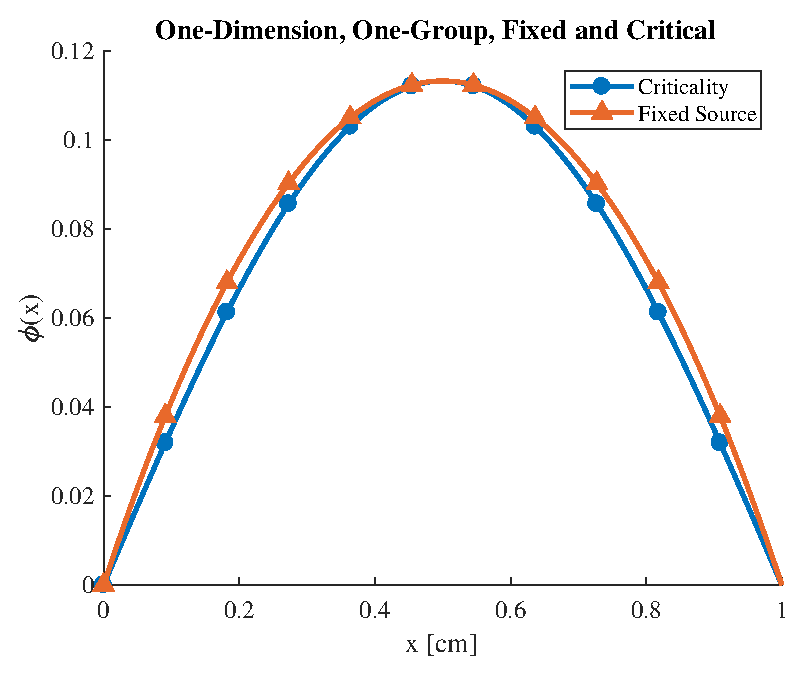
\includegraphics[width=0.7\textwidth]{fixed_critical}
    \caption{Fixed Source and Criticality Flux Shapes for One-Dimension,
      One-Group Problems.}
    \label{fig:fixed_critical}
  \end{figure}
\end{frame}

\begin{frame}{Two-Dimension, One-Group, Criticality}
  \begin{table}
    %\caption{Two-Dimension, One-Group, Criticality Convergence Study
    %  Results.}
    \label{tab:2d1g}
    \begin{center}
      \resizebox{\textwidth}{!}{
      \begin{tabular}{cccccccccc}
        \toprule
        Refine & $\keff$ & $\keff$ error \units{pcm} & $\keff$ ratio & RMS & 
          RMS ratio  & $\|e\|_{\infty}$ & $\|e\|_{\infty}$ ratio \\
        \midrule
        \csvreader[
          late after line=\\,
          late after last line=\\,]
          {../ch03_diffusionResults/data/2d1g.csv}{}
          {\csvcoli & \csvcolii & \csvcoliii & \csvcoliv & \csvcolv & 
          \csvcolvi & \csvcolxi & \csvcolxii}
        Ref. & 1.996060  \\
        \bottomrule
      \end{tabular}
    }
    \end{center}
  \end{table}
  \begin{equation}
    \label{eq:analytic_2d1g}
    \phi(x,y) = \phi_0 \sin\left(\frac{\pi}{L_x} x\right) \, 
      \sin\left(\frac{\pi}{L_y} y\right)
  \end{equation}
\end{frame}

\begin{frame}{Two-Dimension, One-Group, Criticality}
  \begin{figure}
    \centering
    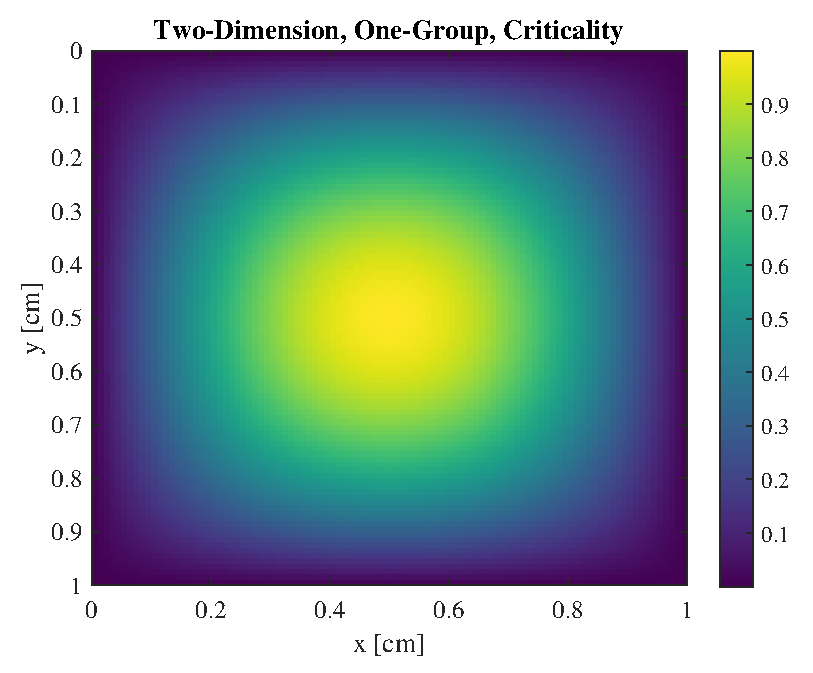
\includegraphics[width=0.7\textwidth]{2d1g}
    \caption{Two-Dimension Criticality Flux Shape.}
    \label{fig:2d1g}
  \end{figure}
\end{frame}

\begin{frame}{One-Dimension, Two-Group, Criticality}
  \begin{table}
    %\caption{One-Dimension, Two-Group, Criticality Convergence Study
    %  Results.}
    \label{tab:1d2g}
    \begin{center}
      \resizebox{\textwidth}{!}{
      \begin{tabular}{ccccccc}
        \toprule
        Refine & $\keff$ & $\keff$ error \units{pcm} & $\keff$ ratio & 
          $\phi_2/\phi_1$ & $\phi_2/\phi_1$ error & $\phi_2/\phi_1$ ratio \\
        \midrule
        \csvreader[
          late after line=\\,
          late after last line=\\,]
          {../ch03_diffusionResults/data/1d2g.csv}{}
          {\csvcoli & \csvcolii & \csvcoliii & \csvcoliv & \csvcolv & 
          \csvcolvi & \csvcolvii}
        Ref. & 0.892349 &  &  & 0.261324 \\
        \bottomrule
      \end{tabular}
    }
    \end{center}
  \end{table}
  \begin{align}
    \phi_1(x) &= \phi_0 \, \sin\left(\frac{\pi}{L_x} x \right), \\
    \phi_2(x) &= \frac{k_2}{k_1} \, \phi_0 \, \sin\left(\frac{\pi}{L_x} x
      \right), \\
    \frac{k_2}{k_1} &= \frac{\Sigma_{s 1\rightarrow 2}}{D_2 \,
      \left(\frac{\pi}{L_x}\right)^2 + \Sigma_{r2}}
  \end{align}
\end{frame}

\begin{frame}{One-Dimension, Two-Group, Criticality}
  \begin{figure}
    \centering
    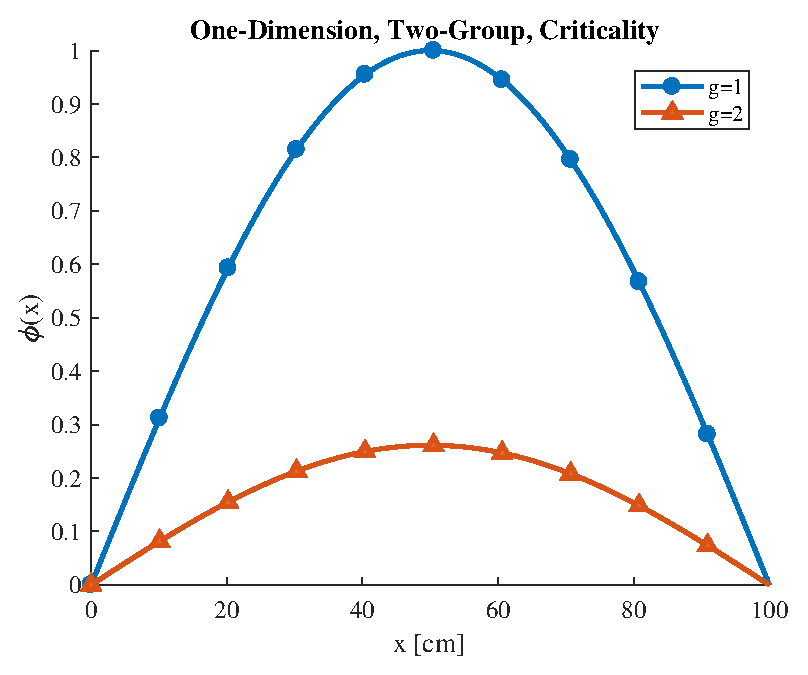
\includegraphics[width=0.7\textwidth]{1d2g}
    \caption{Example Two-Group Flux Plot.}
    \label{fig:1d2g}
  \end{figure}
\end{frame}

\begin{frame}{One-Dimension, One-Group, Two Region, Criticality}
  \begin{table}
    %\caption{One-Dimension, One-Group, Two-Region, Criticality Convergence
    %  Study Results.}
    \label{tab:2reg}
    \begin{center}
      \resizebox{\textwidth}{!}{
      \begin{tabular}{cccccccccc}
        \toprule
        Refine & $\keff$ & $\keff$ error \units{pcm} & $\keff$ ratio & RMS & 
          RMS ratio  & $\|e\|_{\infty}$ & $\|e\|_{\infty}$ ratio \\
        \midrule
        \csvreader[
          late after line=\\,
          late after last line=\\,]
          {../ch03_diffusionResults/data/2reg.csv}{}
          {\csvcoli & \csvcolii & \csvcoliii & \csvcoliv & \csvcolv & 
          \csvcolvi & \csvcolxi & \csvcolxii}
        Ref. & 0.962188 \\
        \bottomrule
      \end{tabular}
    }
    \end{center}
  \end{table}
  \begin{align}
    \phi_F(x) &= \phi_0 \, \cos(B_F \, x) \\
    \phi_R(x) &= \phi_0 \, \cos(B_F \, L_F) \, \cosh(\kappa_R \, (x-L_F)) - 
      \frac{\phi_0 \, D_F \, B_F \, \sin(B_F\,L_F)}{D_R \, \kappa_R} \, 
      \sinh(\kappa_R\,(x-L_F)) \\
    \label{eq:analytic_2reg}
    %\phi(x) &= H(x-L_F) \, \phi_R(x) + H(L_F-x) \, \phi_F(x)
    \phi(x) &=
    \begin{cases}
      \phi_F(x) & 0   \le x \le L_F \\
      \phi_R(x) & L_F \le x \le L_R
    \end{cases}
  \end{align}
\end{frame}

\begin{frame}{One-Dimension, One-Group, Two Region, Criticality}
  \begin{figure}
    \centering
    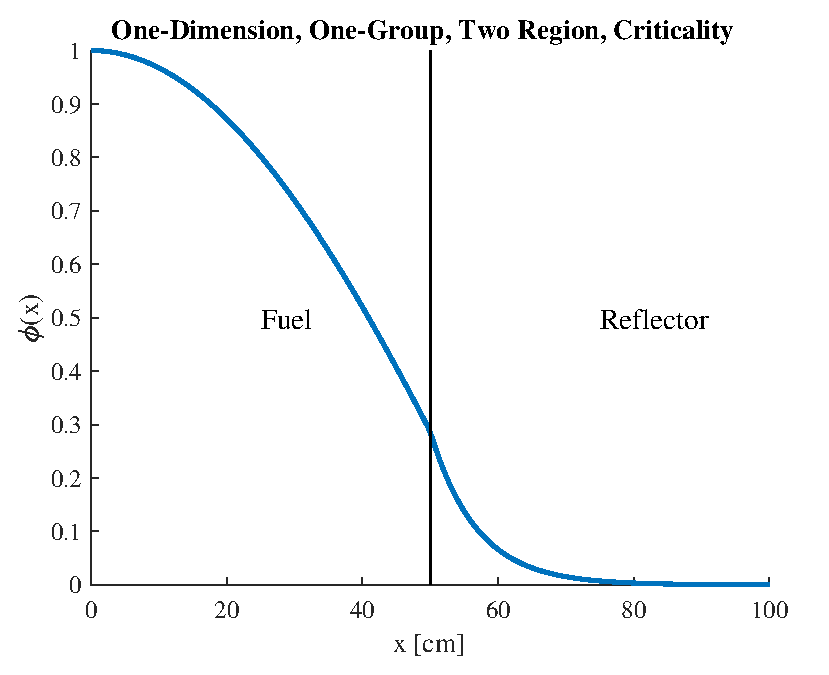
\includegraphics[width=0.7\textwidth]{2reg}
    \caption{Two Region Flux Shape.}
    \label{fig:2reg}
  \end{figure}
\end{frame}

\begin{frame}{Three-Dimension, One-Group, Finite Cylinder}
  \begin{table}
    %\caption{Finite Cylinder Convergence Study Results.}
    \label{tab:finite_cyl}
    \begin{center}
      \resizebox{\textwidth}{!}{
      \begin{tabular}{cccccccccc}
        \toprule
        Refine & $\keff$ & $\keff$ error \units{pcm} & $\keff$ ratio & RMS & 
          RMS ratio  & $\|e\|_{\infty}$ & $\|e\|_{\infty}$ ratio \\
        \midrule
        \csvreader[
          late after line=\\,
          late after last line=\\,]
          {../ch03_diffusionResults/data/finite_cyl.csv}{}
          {\csvcoli & \csvcolii & \csvcoliii & \csvcoliv & \csvcolv & 
          \csvcolvi & \csvcolxi & \csvcolxii}
        Ref. & 0.996711 \\
        \bottomrule
      \end{tabular}
    }
    \end{center}
  \end{table}
  \begin{equation}
    \label{eq:analytic_finite_cyl}
    \phi(r,z) = \phi_0 \, 
      J_0\left(\frac{\alpha_0}{T} r\right) \sin\left(\frac{\pi}{H} z \right)
  \end{equation}
\end{frame}

\begin{frame}{Three-Dimension, One-Group, Finite Cylinder}
  \begin{figure}
    \centering
    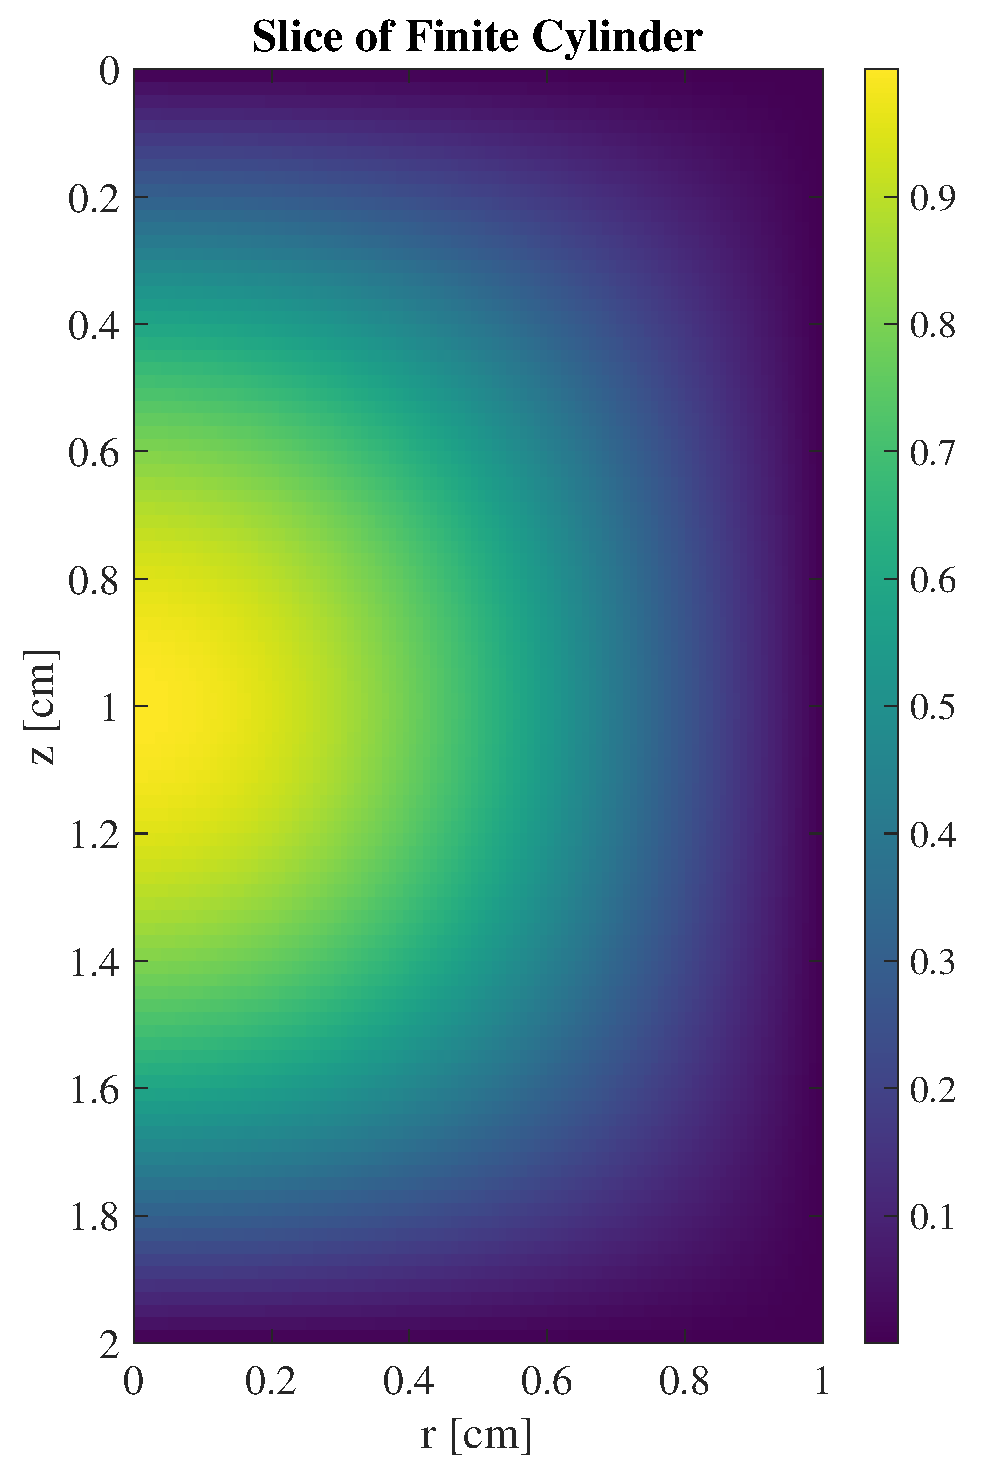
\includegraphics[width=0.4\textwidth]{finite_cyl}
    \caption{Example Finite Cylinder Flux Shape.}
    \label{fig:finite_cyl}
  \end{figure}
\end{frame}
